\section*{ANEXOS}
    %%%%%%%%%%%%%%%%%
    %   EQUAÇÕES    %
    %%%%%%%%%%%%%%%%%

    \begin{eqfloat}[h!]
        \begin{equation}
            P = I * R^{2}
            \label{eq:ganho_tensao}
        \end{equation}
        \caption{Fórmula da potência dissipada por uma carga.}
    \end{eqfloat}
    
    
    %%%%%%%%%%%%%%%
    %   FIGURAS   %
    %%%%%%%%%%%%%%%
    \begin{figure}[h!]
        \centering
        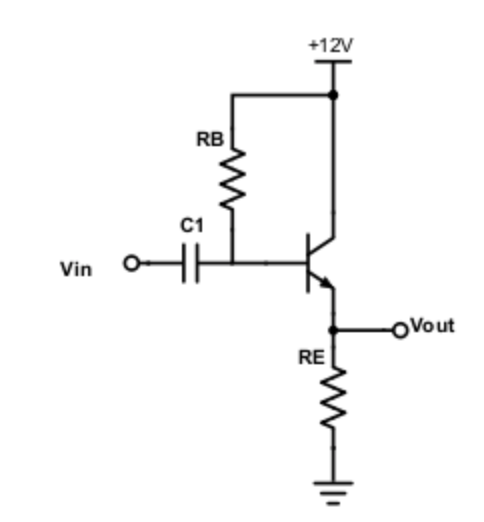
\includegraphics[height=5.5cm]{imgSource/circuitolab4.png}
        \caption{Circuito seguidor de emissor com transístor BJT.}
        \label{fig:circLab4}
    \end{figure}
    
    \begin{figure}[h!]
        \centering
        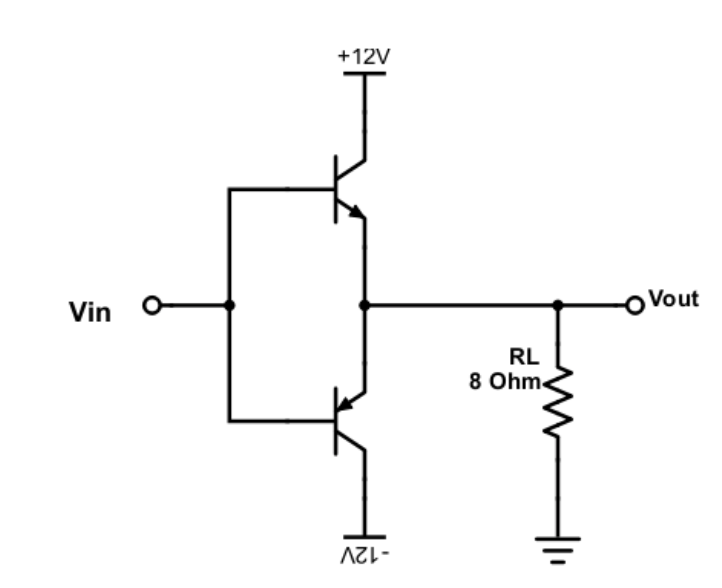
\includegraphics[height=5.5cm]{imgSource/pushPullSimp.png}
        \caption{Circuito \emph{push-pull} simples.}
        \label{fig:pushSimp}
    \end{figure}
    
    \begin{figure}[h!]
        \centering
        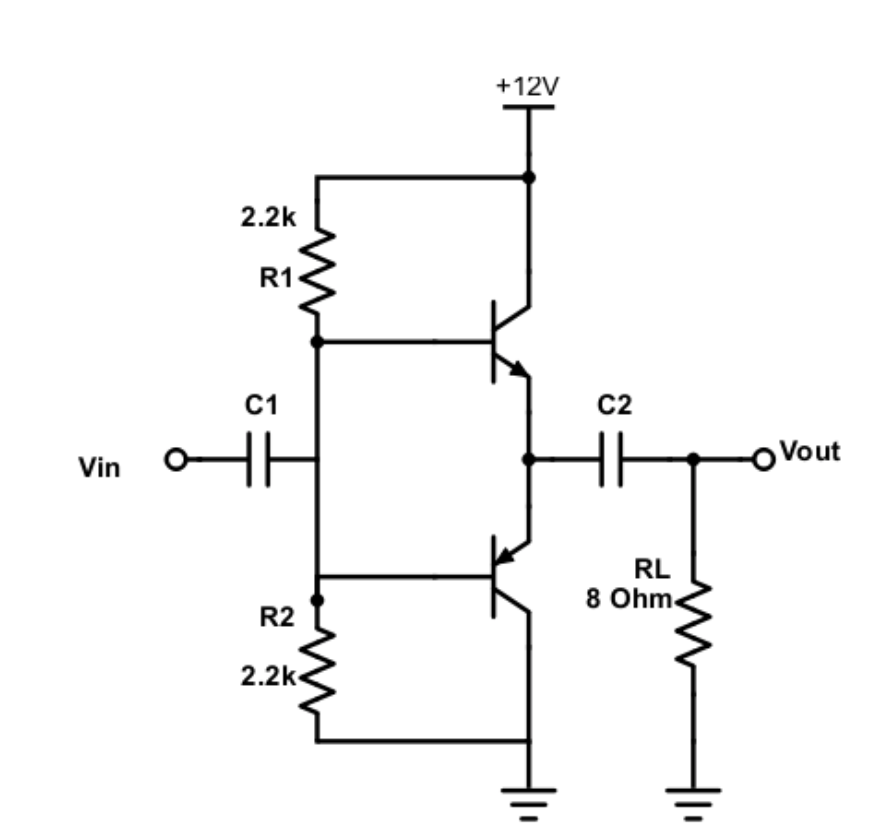
\includegraphics[height=5.5cm]{imgSource/pushPullAssi.png}
        \caption{Circuito \emph{push-pull} simples com alimentação assimétrica.}
        \label{fig:pushAssi}
    \end{figure}
    
    \begin{figure}[h!]
        \centering
        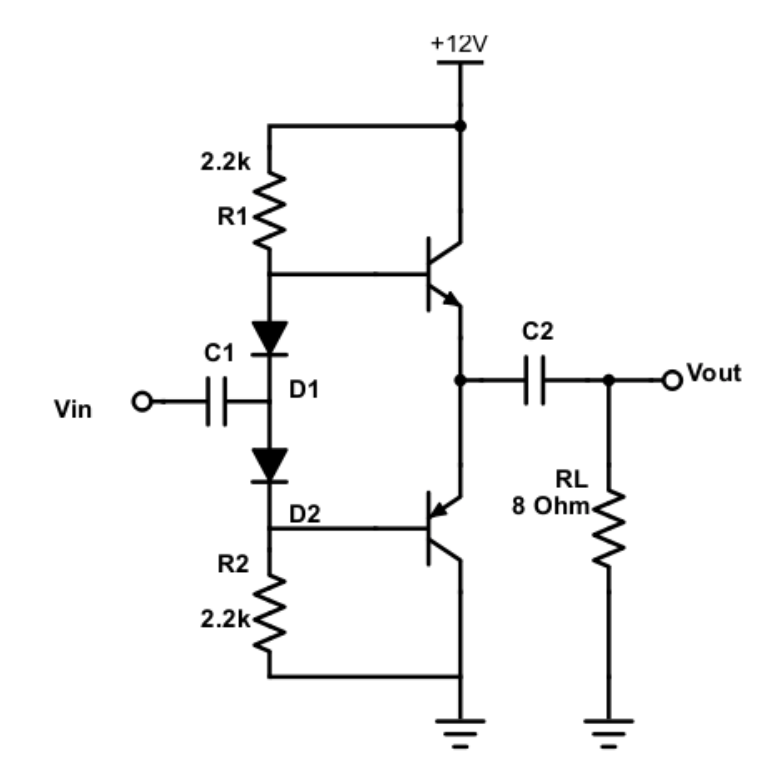
\includegraphics[height=5.5cm]{imgSource/pushPullPol.png}
        \caption{Circuito \emph{push-pull} com polarização e alimentação assimétrica.}
        \label{fig:pushPol}
    \end{figure}
    
    \begin{figure}[h!]
        \centering
        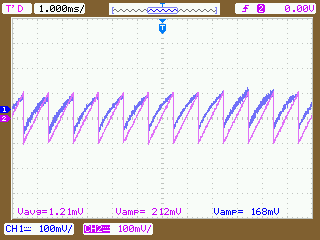
\includegraphics[height=5.5cm]{imgSource/oscilloscope/NewFile0.png}
        \caption{Sinal de saída do circuito push-pull com deformação.}
        \label{fig:newFile0}
    \end{figure}
    
    \begin{figure}[h!]
        \centering
        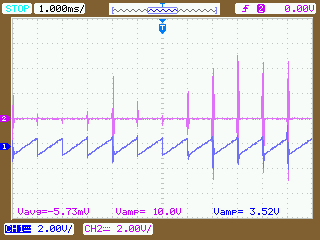
\includegraphics[height=5.5cm]{imgSource/oscilloscope/NewFile4.png}
        \caption{Sinal de saída com a carga (alto-falante) acoplada.}
        \label{fig:newFile4}
    \end{figure}
    
    \begin{figure}[h!]
        \centering
        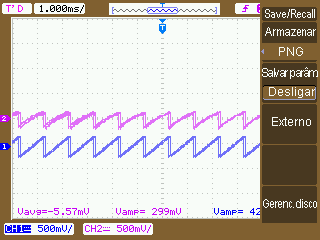
\includegraphics[height=5.5cm]{imgSource/oscilloscope/NewFile5.png}
        \caption{Sinal de saída para sinal de entrada de $200mV_{PP}$.}
        \label{fig:newFile5}
    \end{figure}
    
    \begin{figure}[h!]
        \centering
        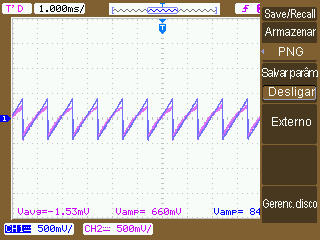
\includegraphics[height=5.5cm]{imgSource/oscilloscope/NewFile6.png}
        \caption{Sinal de saída para sinal de entrada de $400mV_{PP}$.}
        \label{fig:newFile6}
    \end{figure}
    
    \begin{figure}[h!]
        \centering
        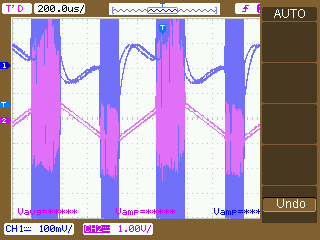
\includegraphics[height=5.5cm]{imgSource/oscilloscope/NewFile7.png}
        \caption{Sinal de saída para o circuito push-pull com entrada assimétrica.}
        \label{fig:newFile7}
    \end{figure}
    
    \begin{figure}[h!]
        \centering
        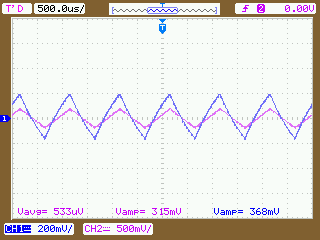
\includegraphics[height=5.5cm]{imgSource/oscilloscope/NewFile8.png}
        \caption{Sinal de saída para o circuito com diodos e entrada de 1KHz.}
        \label{fig:newFile8}
    \end{figure}
    
    \begin{figure}[h!]
        \centering
        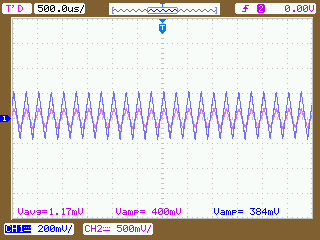
\includegraphics[height=5.5cm]{imgSource/oscilloscope/NewFile9.png}
        \caption{Sinal de saída para o circuito com diodos e entrada de 4KHz.}
        \label{fig:newFile9}
    \end{figure}
    
    \begin{figure}[h!]
        \centering
        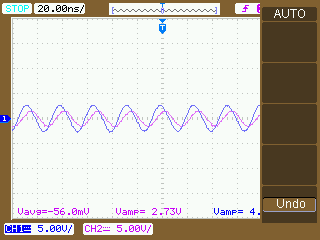
\includegraphics[height=5.5cm]{imgSource/oscilloscope/NewFile10.png}
        \caption{Sinal de saída para o circuito com diodos e entrada de 1KHz e carga (alto-falante acoplado.}
        \label{fig:newFile10}
    \end{figure}
    
    \begin{figure}[h!]
        \centering
        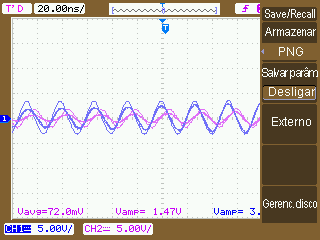
\includegraphics[height=5.5cm]{imgSource/oscilloscope/NewFile11.png}
        \caption{Sinal de saída para o circuito com diodos e entrada de 4KHz e carga (alto-falante acoplado.}
        \label{fig:newFile11}
    \end{figure}